\chapter{Planteamiento del problema y justificación}

\section{Planteamiento del problema}

Las lesiones cutáneas constituyen una de las patologías de mayor prevalencia en la práctica dermatológica y se clasifican en benignas, como los nevos melanocíticos y la queratosis seborreica, y malignas, entre las que destacan el melanoma (MEL), el carcinoma basocelular (BCC) y el carcinoma de células escamosas (SCC). El cáncer de piel es reconocido por la Organización Mundial de la Salud (OMS) como una de las neoplasias más frecuentes, con una incidencia creciente entre 1990 y 2021 \parencite{zhou2025skinburdengbd}. En Colombia, la Cuenta Alto Costo reportó 11.064 casos en 2024 \parencite{elfrente2024cancerpielhic,cuentaaltocosto2025melanoma}, en un país cuya cercanía al ecuador implica una exposición elevada a la radiación ultravioleta \parencite{oliveros2025melanomacolombia}.
A nivel nacional, un estudio con los casos nuevos de melanoma reportados en 2019 al Sistema Integral de Información de la Protección Social (SISPRO) encontró que la incidencia depende de la altitud, usada como indicador de exposición a radiación ultravioleta (UV): 7,7 casos por 100.000 habitantes entre 0 y 400 m, frente a 17,52 entre 1.801 y 3.000 m, con un rango regional de 0,6 a 53 \parencite{oliveros2025melanomacolombia}. Los autores sugieren que las menores tasas a baja altitud podrían corresponder al predominio de los fototipos III y IV en las costas Pacífica y Caribe. En Santander, el Instituto de Cáncer del HIC registra 3.060 casos entre 2016 y 2023, con predominio del BCC (64,82\%); el melanoma, pese a representar solo el 13,66\% de los casos, causó el 80\% de las muertes \parencite{uribe2018bccbucaramanga}.
Tradicionalmente, estas lesiones se identifican mediante el método ABCDE (asimetría, borde, color, diámetro y evolución) apoyado en imágenes dermatológicas, pero su precisión depende de la experiencia del especialista: cerca de 62\% en dermatólogos con 3 a 5 años de práctica y hasta 80\,\% con más de 10 \parencite{chaturvedi2020multiclassskin}. Los casos complejos requieren biopsia, un procedimiento invasivo, costoso y demorado \parencite{pathania2022noninvasivediagnostics,sauter2023dermatopathologyreview}, lo que dificulta el diagnóstico oportuno en regiones como Santander.
Con el objetivo de apoyar la labor clínica, se han desarrollado sistemas de diagnóstico asistido por computador (CAD) basados en aprendizaje profundo, con desempeños comparables al de especialistas en la clasificación de lesiones cutáneas sobre conjuntos como HAM10000, ISIC y DermNet \parencite{omiye2025reflectanceconfocal,tschandl2018ham10000}. Su implementación en contextos como el colombiano enfrenta dos barreras. La primera es la escasez de datos etiquetados: entrenar un modelo supervisado requiere imágenes con diagnóstico confirmado por especialistas, y producir esas anotaciones demanda tiempo clínico y recursos que los hospitales no siempre pueden destinar a ello \parencite{wang2023pymic}. La segunda es el cambio de dominio, que ocurre cuando las imágenes de entrenamiento difieren de aquellas en las que el modelo se usa después. HAM10000, por ejemplo, se recopiló en Austria y Australia \parencite{tschandl2018ham10000}, con poblaciones, equipos y protocolos de captura que pueden diferir de los de otros contextos, y la variedad de pigmentaciones y texturas de la piel sigue siendo un reto para la generalización de los modelos
En este contexto, las técnicas de aprendizaje autosupervisado se presentan como una alternativa prometedora en el análisis de imágenes médicas, al permitir el entrenamiento de modelos utilizando grandes volúmenes de datos no etiquetados. Este enfoque reduce significativamente la dependencia de conjuntos de datos anotados y ha mostrado resultados alentadores en diferentes tareas de diagnóstico asistido por imágenes \parencite{krishnan2022selfsupervisedmedicine}. Por lo tanto, su aplicación en el análisis de imágenes dermatológicas podría contribuir al desarrollo de herramientas computacionales que apoyen la detección y clasificación de lesiones cutáneas, fortaleciendo las capacidades diagnósticas en contextos regionales como el departamento de Santander.

\subsection*{Árbol del problema}
\begin{figure}[htbp]
\centering
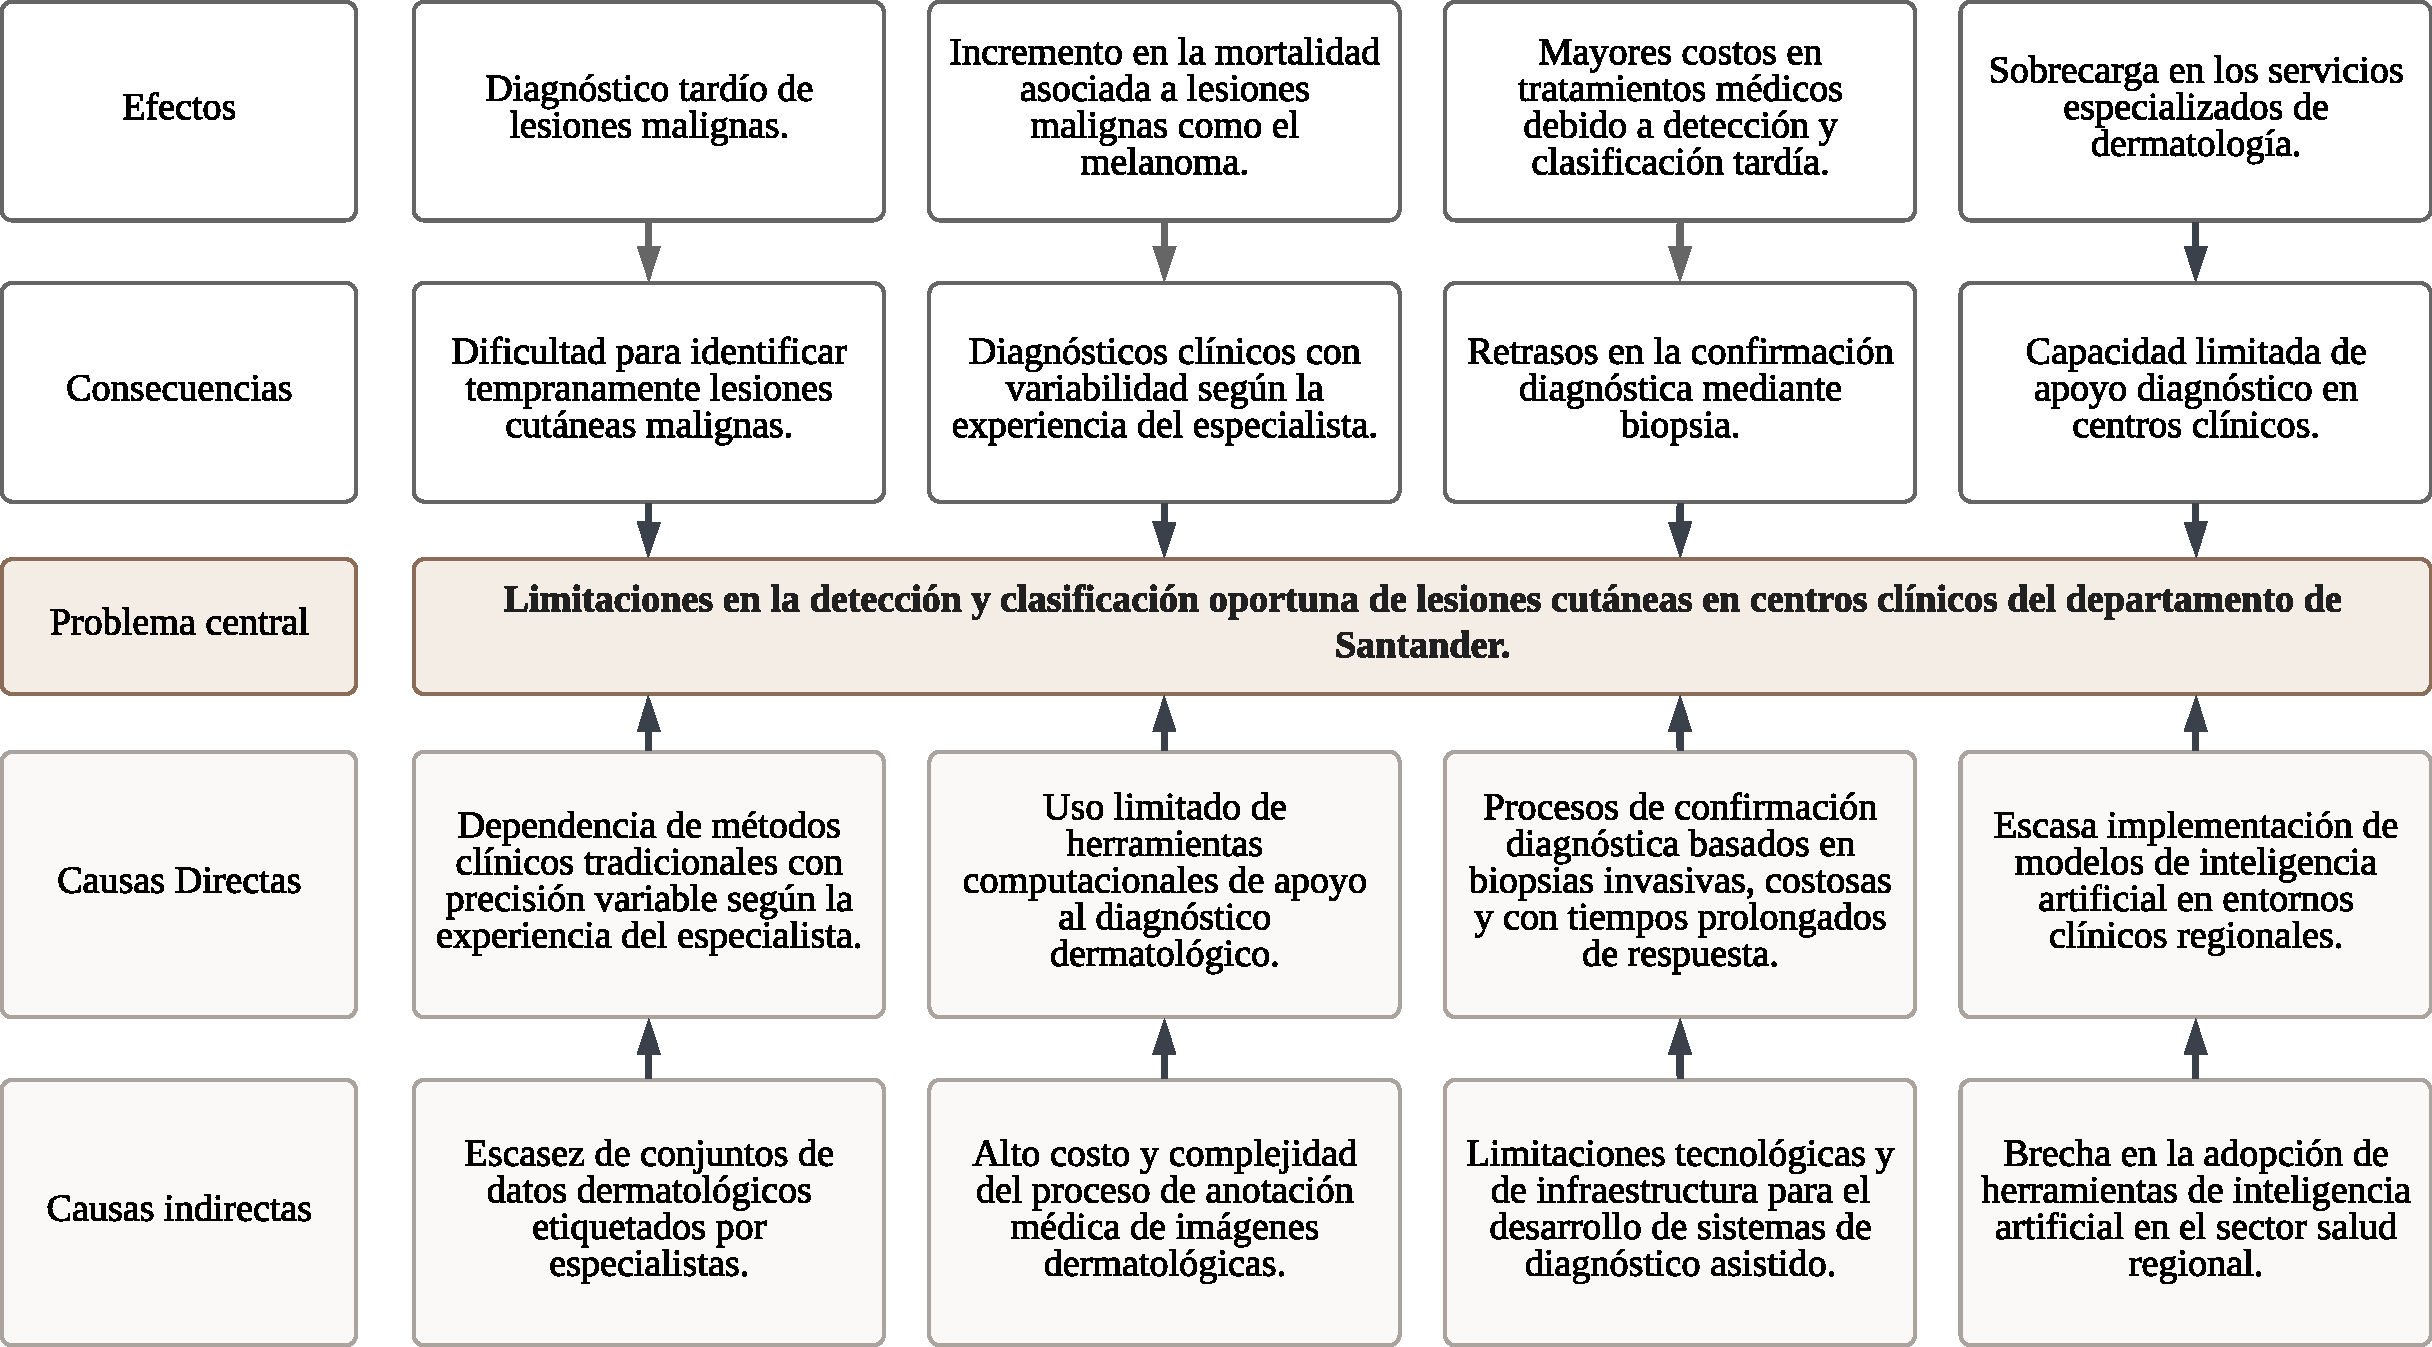
\includegraphics[width=\textwidth]{images/arbol-problema.pdf}
\caption{Árbol del problema de clasificación de lesiones cutáneas.}
\label{fig:arbol-problema}
\end{figure}

\subsection{Pregunta de investigación}

¿Cómo diseñar un algoritmo de inteligencia artificial basado en aprendizaje autosupervisado para clasificar lesiones cutáneas a partir de imágenes dermatológicas y apoyar el análisis clínico en el contexto del departamento de Santander?

\section{Justificación}

La integración de la inteligencia artificial en los procesos de diagnóstico clínico constituye uno de los avances más significativos en la ingeniería aplicada al sector salud. No obstante, la mayoría de los modelos de inteligencia artificial desarrollados hasta la fecha han sido concebidos y validados en contextos con infraestructuras tecnológicas consolidadas y con acceso a grandes volúmenes de datos clínicos previamente anotados por especialistas. Esta condición limita su aplicabilidad en sistemas de salud con características diferentes, como el colombiano, donde la disponibilidad de conjuntos de datos etiquetados suele ser reducida y los recursos para su generación son limitados.

En este contexto, el presente proyecto responde a una necesidad identificada en el ámbito clínico regional, particularmente en el apoyo al diagnóstico de lesiones cutáneas mediante herramientas tecnológicas que complementen la evaluación médica. Asimismo, se alinea con los lineamientos de transformación digital en salud promovidos por el Ministerio de Salud y Protección Social de Colombia, los cuales reconocen el desarrollo de soluciones basadas en inteligencia artificial como una estrategia para fortalecer las capacidades diagnósticas y reducir brechas en el acceso a tecnologías médicas a nivel territorial \parencite{yang2024crosshospital}.

El aporte diferencial de esta investigación radica en la exploración de enfoques de aprendizaje automático que reduzcan la dependencia de grandes volúmenes de datos anotados. En particular, el aprendizaje autosupervisado permite aprovechar conjuntos de datos no etiquetados para el entrenamiento de modelos capaces de extraer representaciones relevantes de las imágenes, lo que lo convierte en una alternativa viable para contextos donde la disponibilidad de anotaciones clínicas es limitada. Este enfoque no solo resulta pertinente para el contexto local, sino que también puede ser replicado en otras instituciones de salud que enfrentan condiciones similares de acceso a datos médicos anotados \parencite{hammimou2025skinsegmentationreview}.

La viabilidad del proyecto se sustenta en la disponibilidad de conjuntos de datos dermatológicos ampliamente utilizados en la investigación científica y en el desarrollo reciente de técnicas de aprendizaje autosupervisado para el análisis de imágenes médicas. Estos enfoques han demostrado resultados prometedores en tareas de clasificación y detección, lo que respalda su potencial aplicación en el desarrollo de herramientas computacionales de apoyo al diagnóstico dermatológico \parencite{chaturvedi2020multiclassskin}.

Finalmente, el desarrollo de este proyecto contribuye al fortalecimiento de competencias en áreas como el diseño de sistemas inteligentes, el procesamiento y análisis de imágenes médicas y la implementación de modelos de aprendizaje automático, promoviendo una formación orientada hacia la innovación tecnológica con impacto potencial en el mejoramiento de los procesos de diagnóstico clínico.
